\documentclass[10pt]{article}
\usepackage[margin=0.9in]{geometry}
\usepackage[utf8]{inputenc}
\usepackage{amsmath,amssymb,booktabs,graphicx,hyperref,xcolor}
\usepackage[numbers]{natbib}
\hypersetup{colorlinks=true,linkcolor=blue!50!black,citecolor=blue!50!black,urlcolor=blue!50!black}
\graphicspath{ {../docs/figures/} }
\title{Holes in Neural Geometry: Exact Topology of Fitted Shapes and Persistent Homology\\of Top-3-PCA Activation Clouds, and Whether Cyclic Concepts Travel Around Them}
\author{Libor ``Burny'' Burian}
\date{15 November 2026}
\begin{document}
\maketitle

\begin{abstract}
Interpretability work reports circles, helices and other low-dimensional shapes in neural activations, usually identified by eye or by fitting. We ask the topological question behind a common hypothesis: does a concept have a \emph{hole} you can travel around, and does its semantic cycle go around it exactly once? The motivation is manifold steering~\citep{wurgaft2026manifold}: if so, steering around the loop should be semantically meaningful.

We study the 44 top-3-PCA activation and weight clouds of a sibling shape-fitting project~\citep{shapefitting2026}, which come from GPT-2, Llama-3.1-8B, Pythia, a grokked modular-addition transformer and controls. We use two independent methods.
\textbf{(A)} The fitted shapes are uniquely parametrised, so their Betti numbers, Euler characteristic and genus are exact. A margin ratio $\rho_A$ measures whether the data resolve that topology.
\textbf{(B)} Alpha-complex persistent homology with design-matched Monte Carlo nulls, and circle-valued coordinates from persistent cohomology.

Colour hue, residues mod 113 and months have significant holes. The Monte Carlo $p$-values of the loop test are 0.001, 0.001 and 0.002 (999 null draws). The concept goes around each hole once in 3D; for months this holds only in a post hoc analysis. Only the colour loop persists beyond the top-3 PCs.
Weekdays have no detectable hole ($p = 0.094$), although the days are ordered around the axis of their fitted helix (exact $p = 0.003$).
No ordinal concept and none of 20 random-process controls has a hole.
The fitter's ``helix'' labels for cyclic concepts hide closed loops: their openness is within noise ($\rho_A \approx 0.11$), and for months the axial position is a second Fourier harmonic, which makes the curve a closed saddle loop (post hoc).

The strict preregistered conjunctions pass for none of the three primary cyclic sets: 0/3 by fitted-shape topology and 0/3 by persistent homology. Specificity holds.
On 39{,}000 synthetic clouds with exact ground-truth topology, the preregistered estimator recovers the exact Betti vector for 0.618 of resolvable clouds (macro). Reading topology from the fitter's family label scores 0.812, but persistent homology wins when topology is well resolved (0.94 vs 0.86).
Steering experiments are preregistered and postponed.
\end{abstract}

\section{Introduction}

Low-dimensional shapes in activations are a recurring finding.
\begin{itemize}
  \item Circles for weekdays and months~\citep{engels2025notall}.
  \item A helix of GPT-2 positions~\citep{yedidia2023helix}.
  \item Circles of residues in grokked modular addition~\citep{nanda2023progress}.
  \item Loops for colours and dates~\citep{modell2025origins}.
\end{itemize}
Manifold steering~\citep{wurgaft2026manifold,goodfire2026geometry} moves activations along a fitted manifold. On a weekday manifold this shifts the output from Monday to Tuesday and so on, whereas linear steering cuts across the manifold.

These works identify shapes geometrically. A geometric label such as ``helix'' does not say whether a concept has a \emph{hole}, a 1-cycle in homology, or whether the semantic order goes \emph{around} it. That is what would make steering around a loop meaningful.

\paragraph{Contributions.}
\begin{enumerate}
  \item The exact topology of every fitted shape: Betti numbers, $\chi$, genus, boundary components. A margin ratio $\rho_A$ tests resolvability. We also read out the intrinsic coordinates of every labelled point on its fitted shape.
  \item A preregistered, null-controlled persistent-homology test of whether cyclic concepts have a hole that their semantic order travels around once. It uses design-matched nulls, a projection-robustness check, and ordinal and random-init negative controls.
  \item A validation of persistent-homology Betti estimators against exact ground truth on 39{,}000 synthetic clouds of 13 families.
  \item Everything is reproducible from GitHub and Hugging Face, and every number is generated from results files.
\end{enumerate}

\section{Related work}

\paragraph{Topology of neural representations.}
\begin{itemize}
  \item Layer-wise topology simplification~\citep{naitzat2020topology}.
  \item Zigzag persistence across LLM layers~\citep{gardinazzi2025persistent}.
  \item Betti numbers of modular-addition representations~\citep{moisescu2025modular} and H1 at grokking~\citep{tang2026grokking}. Neither uses a null model.
  \item A persistence ratio for small centroid clouds of imposed cycles~\citep{david2026context}.
\end{itemize}

\paragraph{Neuroscience.} Ring and torus detection uses shuffle nulls and circular-coordinate decoding~\citep{chaudhuri2019intrinsic,gardner2022toroidal}. Circular coordinates themselves come from persistent cohomology~\citep{desilva2011circular,perea2023dreimac}.

\paragraph{Inference.} The universal null~\citep{bobrowski2023universal} gives per-bar $p$-values. Max-over-null Monte Carlo thresholds~\citep{gardner2022toroidal} are the practical standard.

\paragraph{Pitfalls.} PCA horseshoes and Lissajous loops~\citep{antognini2018pca,shinn2023phantom}, and Rips phantom classes~\citep{adamaszek2017rips}.

\paragraph{Gap.} We found no work that tests, with a null model, whether a cyclic concept's representation has a 1-cycle aligned with its semantic order. We also found none that compares the exact topology of fitted parametric shapes with persistent homology of the same clouds.

\section{Data}

The 44 clouds of~\citep{shapefitting2026} (commit 4c5f3b6):
\begin{itemize}
  \item Llama-3.1-8B hidden states: weekdays and months at the concept token, layer 5; days-with-times, colours, years, temperatures and ages at the last token, layer 19; city truth statements, layer 12; line-break character counts, layer 5.
  \item Pythia-410m character counts.
  \item Weight matrices: GPT-2 positional embeddings and the embedding of a grokked modular-addition transformer.
  \item Toy models of superposition~\citep{elhage2022toy}.
  \item Controls: 20 Gaussian-process and random-walk ordinal processes, and random-init networks.
\end{itemize}
Each cloud is normalised by the source's \texttt{fit\_frame}: centre, top-3 eigenvectors, skewness signs, RMS radius 1. Our numpy re-implementation reproduces the stored points to $10^{-4}$.

The synthetic test set (39{,}000 clouds, 13 families, 5--1024 points, 3 noise levels) and its validation stream are regenerated bit-exactly on CUDA, together with their ground-truth parameters (maximum difference 0.0).

\section{Method}
\begin{figure}[t]\centering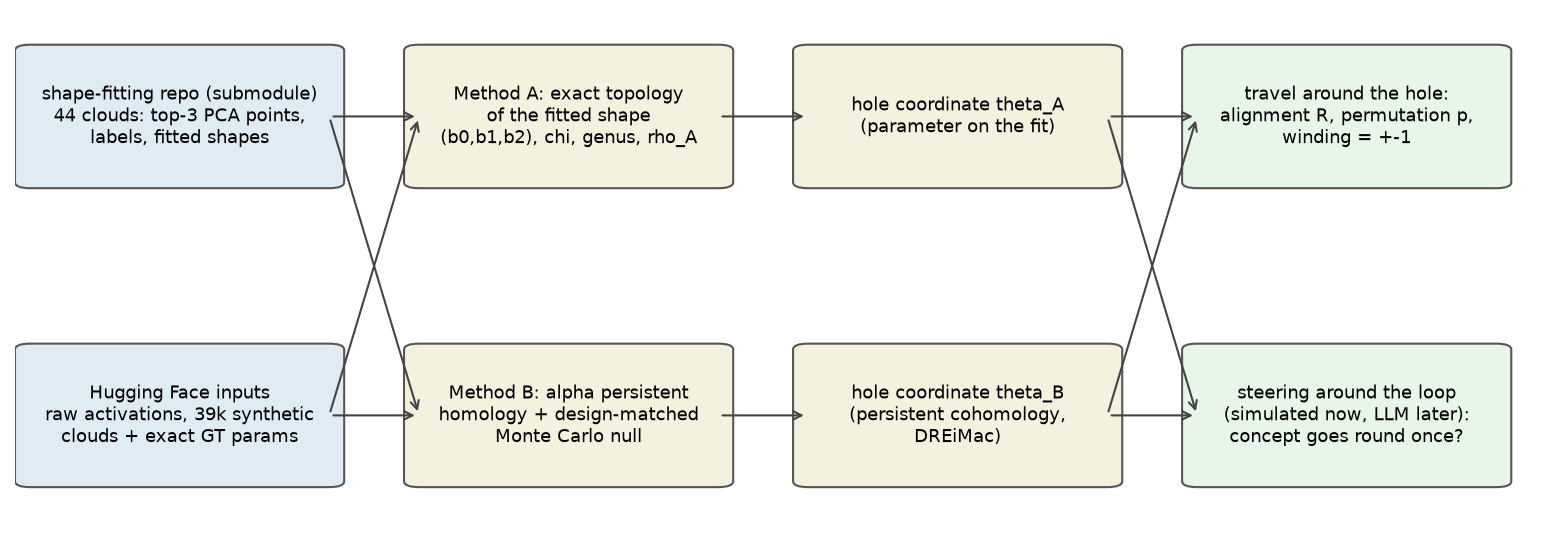
\includegraphics[width=\linewidth]{fig_pipeline.png}
\caption{Pipeline. Method A reads exact topology and point coordinates off the fitted shape; Method B measures persistent homology of the cloud. Both give a circle-valued coordinate for the travel-around-the-hole test. Steering is designed and postponed.}\label{fig:pipeline}\end{figure}

\paragraph{Method A.} Each family is a known space~\citep{hatcher2002algebraic}:
\begin{itemize}
  \item closed arc or ellipse: $S^1$;
  \item helix, line, ringing curve: contractible curves;
  \item disc, paraboloid, spherical cap: discs;
  \item closed sphere: $S^2$;
  \item cone frustum: an annulus;
  \item torus: $T^2$ (genus 1);
  \item clusters and polytopes: point sets.
\end{itemize}
The margin $m$ is the smallest parameter change that alters the topology (for example, a helix's endpoint gap). Its ratio to the noise-and-coverage scale $\nu$ is $\rho_A = m/(2\nu)$; the topology is resolvable if $\rho_A \ge 1$.

Every point gets the parameter of its nearest point on the fit: curve parameter, azimuth, height, or nearest centroid. The rules agree with persistent homology of dense noise-free samples for 0.970 of 234 shapes.

\paragraph{Method B.} Alpha complexes in $\mathbb{R}^3$, which are exact \v{C}ech and free of Rips phantom classes~\citep{desilva2007coverage,adamaszek2017rips}, computed with GUDHI~\citep{gudhi}; Rips complexes with ripser~\citep{tralie2018ripser}.

A bar is significant if its persistence ratio $\pi = \text{death}/\text{birth}$ exceeds the 95th percentile of the maximum $\pi$ over 999 draws of a design-matched null. Every draw passes through the same normalisation.
\begin{itemize}
  \item Prompt-template designs use a cluster-centre null: concept means are redrawn from a Gaussian matched to the covariance of the means, and within-concept residuals are kept.
  \item One-point-per-value designs use a full-dimensional matched Gaussian.
\end{itemize}

\paragraph{Travel around the hole.} The hole coordinate $\theta$ is either the fitted shape's azimuth ($\theta_A$) or DREiMac's circular coordinate of the most persistent class ($\theta_B$; prime 47, at most 200 landmarks, \texttt{standard\_range}).
\begin{itemize}
  \item Concept circular means $\bar\theta_c$, with semantic phases $\phi_c = 2\pi c/n$.
  \item Alignment $R=\max_{s=\pm1}|\frac1n\sum_c e^{i(\bar\theta_c - s\phi_c)}|$, with a permutation null over concept labels (exact for $n=7$; $p_{\min}=1/360$).
  \item The winding number of the semantic cycle in $\theta$.
  \item For residues, the maximum over Fourier frequencies $k$.
\end{itemize}

\paragraph{Preregistration.} The hypotheses, nulls and decision rules were pushed before any topology was computed. Amendment A2, which makes steering the primary hypothesis, was pushed before any persistent homology of real data. Deviations D1--D5 are logged with dates.

\section{Results}

\subsection{Instrument validation (synthetic, exact ground truth)}
Table~\ref{tab:exp1} reports the results. The preregistered estimator (alpha + universal null) is calibrated but conservative.
\begin{itemize}
  \item It is worse than a validation-tuned fixed threshold and than the family-implied baseline. The paired difference vs the family label is -0.194 [-0.203, -0.185].
  \item Persistent homology is better exactly where the family label is topologically ambiguous: open vs closed arcs (0.79 vs 0.58) and caps vs full spheres (0.76 vs 0.61).
  \item It is also better wherever $\rho_A \ge 4$ (Fig.~\ref{fig:rho}).
  \item Tori and thin ellipses are its weak points.
\end{itemize}

\begin{table}[t]\centering\small
\begin{tabular}{lcc}\toprule
Estimator & exact $(b_0,b_1,b_2)$ accuracy [95\% CI] & role\\\midrule
P: alpha + universal null & 0.618 [0.610, 0.626] & preregistered method\\
S: Rips H1 + universal null & 0.660 [0.651, 0.670] & secondary (D1)\\
MC: 3D matched-Gaussian null (3{,}120 subset) & 0.594 [0.561, 0.629] & secondary\\
Ba: fixed $\pi$ thresholds & 0.714 [0.703, 0.725] & baseline\\
Bb: fitter's family $\rightarrow$ modal Betti vector & 0.812 [0.807, 0.816] & baseline\\
Bc: majority vector & 0.555 [0.553, 0.557] & control\\\bottomrule
\end{tabular}
\caption{Exp1: macro-averaged exact Betti-vector accuracy on 30114 resolvable synthetic clouds. CIs are a cluster bootstrap over generator chunks.}\label{tab:exp1}\end{table}

\begin{figure}[t]\centering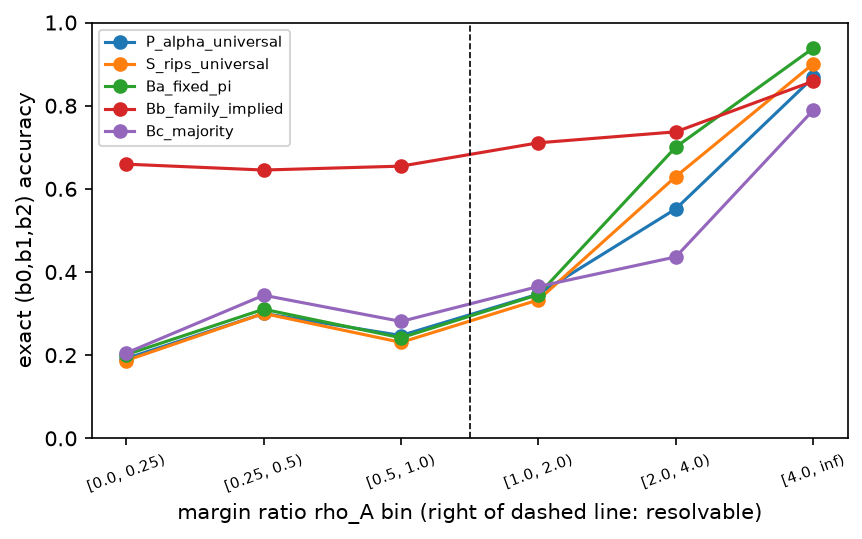
\includegraphics[width=0.62\linewidth]{fig_exp1_by_rho.png}
\caption{Accuracy against the margin ratio $\rho_A$ (all synthetic clouds).}\label{fig:rho}\end{figure}

\subsection{Exact topology of the fitted shapes}
\begin{itemize}
  \item 2 of 44 fits have a hole (cones for years and colours) and 1 has a void (GPT-2 W$_\text{pos}$, a closed sphere). 27 of 44 fitted topologies are resolvable.
  \item The three primary cyclic sets are helices with $\rho_A = 0.11, 0.11, 0.23$, so their openness is not resolvable. H1-A passes 0/3.
  \item The concepts sit around the helix axis in order:
  \begin{itemize}
    \item weekdays: $R=0.83$, exact $p=0.003$, winding 1;
    \item months: $R=0.93$;
    \item residues: $R=0.98$.
  \end{itemize}
  \item Position along the helix does not track the concept order (weekdays $\rho=0.00$).
  \item This winding is not specific: 8 of 8 Gaussian-process controls fitted as helices wind too. The closure gap separates them (Fig.~\ref{fig:helix}): months 0.04 radii, controls 0.33--2.20.
  \item Post hoc, the months' axial position is a second Fourier harmonic of the month angle ($R^2=0.83$ vs 0.10 for the first). The months lie on a closed saddle loop.
  \item Ordinal concepts lie along open curves (counting $\rho=0.999$, temperature -0.997).
\end{itemize}

\begin{figure}[t]\centering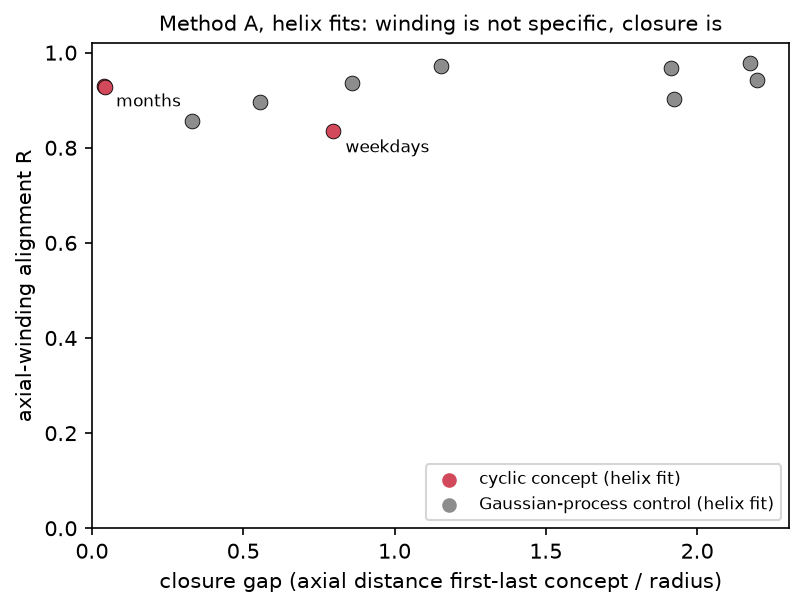
\includegraphics[width=0.55\linewidth]{fig_exp0_helix.png}
\caption{Helix fits: axial-winding alignment is high for cyclic concepts and for smooth random-process controls alike. Closure distinguishes them.}\label{fig:helix}\end{figure}

\subsection{Holes in the data and the cyclic tests}
Table~\ref{tab:real} and Fig.~\ref{fig:gallery} summarise the results.
\begin{itemize}
  \item Significant loops: colours, residues, months, and (unstably) days-with-times.
  \item Weekdays, all six ordinal concepts and all 20 random-process controls have none.
  \item H1-B passes 0/3:
  \begin{itemize}
    \item weekdays fail at the loop step;
    \item months fail at the coordinate step (DREiMac's \texttt{standard\_range} requires a Rips death/birth ratio $\ge 2$);
    \item residues fail only the top-10-PC check.
  \end{itemize}
  \item Specificity (H2): not falsified.
  \item Post hoc, with \texttt{standard\_range=False}, the months wind once around their loop in 3D ($R=0.72$). Colours wind once in 3D and in the top-10 PCs ($R=0.97$). No non-cyclic record winds.
  \item Only the colour loop persists beyond the projection: Rips $\pi$ = 2.67 in 10 PCs and 4.22 in full-dimensional cosine distance.
\end{itemize}

\begin{table}[t]\centering\small
\begin{tabular}{lccccc}\toprule
Dataset & top H1 $\pi$ & null q95 & $p$ & traversal $R$, winding (3D) & Rips $\pi$ top-10 PCs\\\midrule
colours (hue) & 5.02 & 2.38 & 0.001 & 0.95, -1 & 2.67\\
residues mod 113 & 2.45 & 1.83 & 0.001 & 0.97, -1 & 1.16\\
months & 1.72 & 1.44 & 0.002 & 0.72, 1 (post hoc) & 1.13\\
weekdays & 1.32 & 1.36 & 0.094 & -- & 1.22\\
years & 1.63 & 1.94 & 0.775 & -- & 1.39\\
GPT-2 positions & 1.22 & 2.16 & 1.000 & -- & 1.01\\\bottomrule
\end{tabular}
\caption{Method B on key clouds. The null is design-matched (999 draws); traversal uses the cohomology coordinate $\theta_B$.}\label{tab:real}\end{table}

\begin{figure}[t]\centering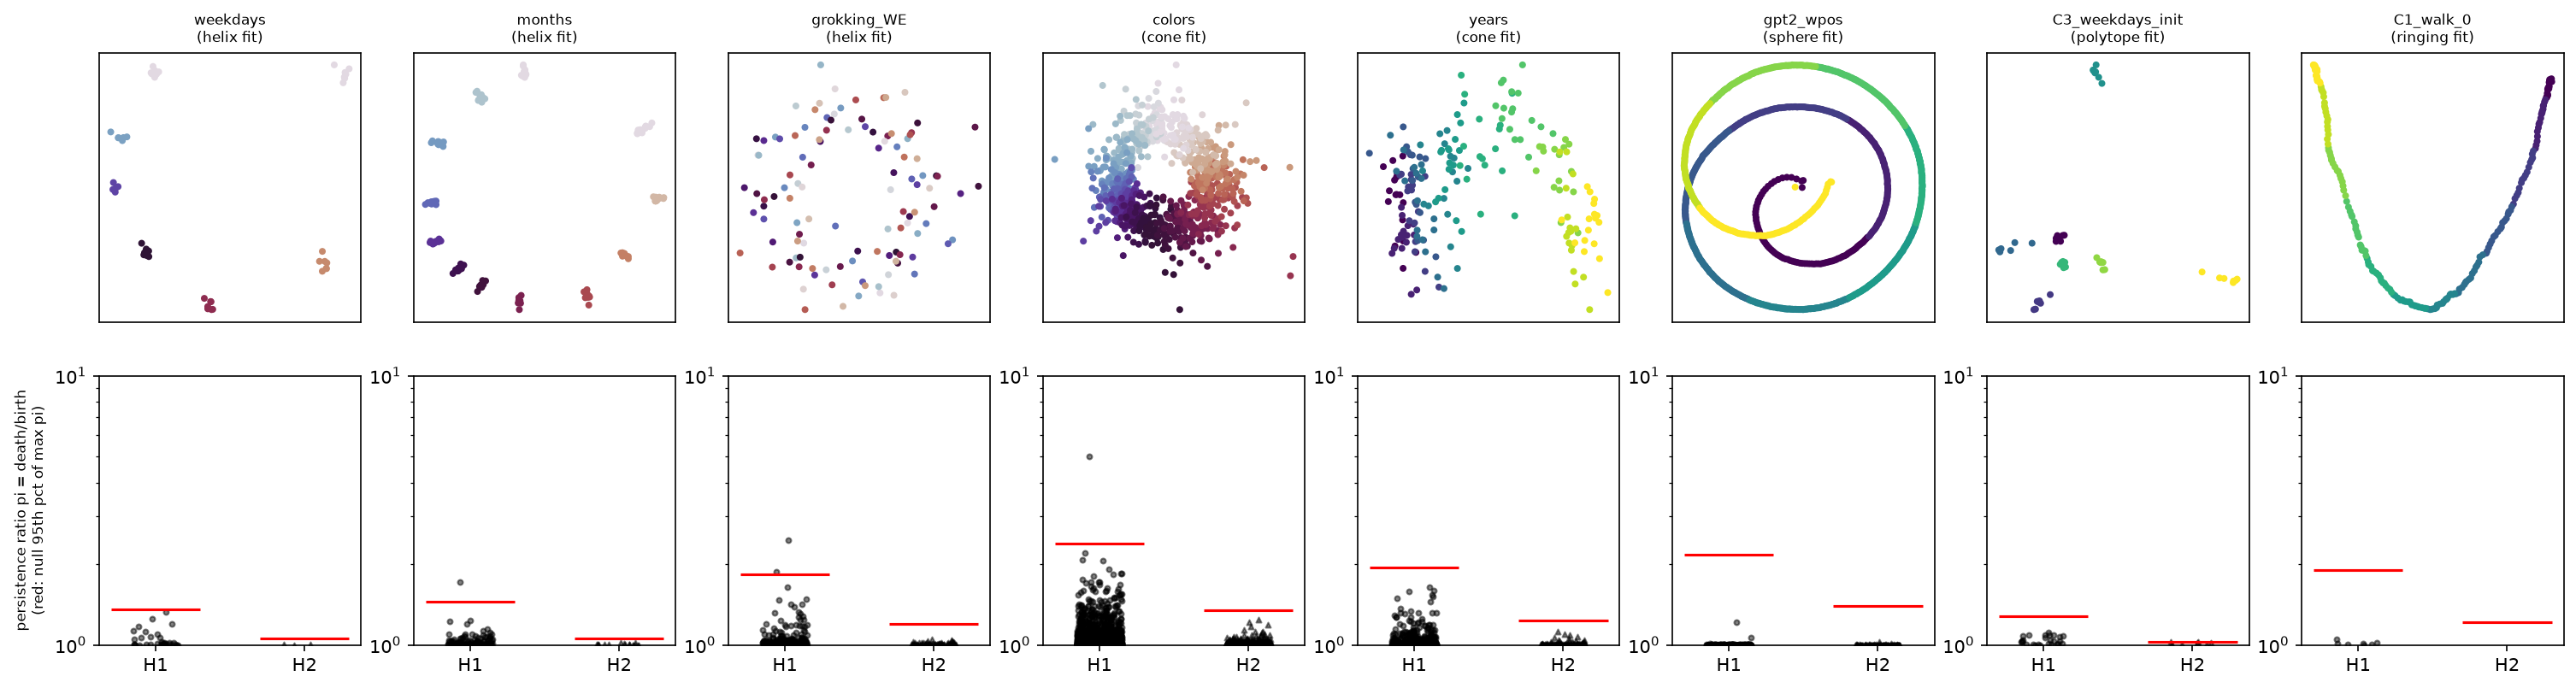
\includegraphics[width=\linewidth]{fig_real_gallery.png}
\caption{Top: clouds (PC1--PC2) coloured by concept. Bottom: alpha persistence ratios with the null 95th percentile (red).}\label{fig:gallery}\end{figure}

\section{Discussion}

\paragraph{Answering the question.}
\begin{itemize}
  \item Topology finds holes exactly for concepts that are semantically cyclic, and never for ordinal concepts or controls. Where a hole exists, the concept goes around it once (months post hoc).
  \item The fitter's helices for cyclic concepts are closed loops within noise.
  \item Whether steering \emph{around} these loops is semantically meaningful is the causal question. It is designed and preregistered (amendment A2), and postponed by the author.
  \item The strongest candidate is colour: a robust loop that hue traverses even outside the top-3 PCs. Months and residues are candidates in the top-3 subspace.
  \item Weekdays show that ``ordered around a circle'' does not guarantee ``topologically detectable hole'' with 7 clusters.
\end{itemize}

\paragraph{Limitations.}
\begin{itemize}
  \item A convenience sample of 44 clouds, with claims made per dataset.
  \item Not blind: the source's labels and figures were known.
  \item The power for 7 clusters is bounded ($\pi \le 1/\sin(\pi/7)$).
  \item DREiMac's \texttt{standard\_range} criterion decided the months verdict.
  \item Exp4 bottleneck similarity was uninformative.
  \item Synthetic accuracy for tori is near zero at these sample sizes.
  \item No causal evidence yet.
\end{itemize}

\section{Conclusion}
Holes found by topology line up with semantically cyclic concepts (colour, residues, months) and are absent for ordinal concepts and controls. Fitted ``helices'' for cyclic concepts are closed loops within noise. Steering around the detected loops is the next, preregistered experiment.

\paragraph{Reproducibility.} Code: \url{https://github.com/BurnyCoder/topology-of-neural-geometry-in-llm-mechanistic-interpretability}. Inputs and results (pinned, SHA-256-verified): \url{https://huggingface.co/datasets/BurnyCoder/topology-of-neural-geometry}. Running \texttt{uv run python run.py all} recomputes every number on a CPU.

\paragraph{AI statement.} Claude Code (Anthropic) wrote this codebase and this paper, executing an exact specification provided by a human author. Human cleanup and rewriting are in progress.

\bibliographystyle{plainnat}
\bibliography{references}
\end{document}
